\documentclass{article}
\usepackage[left=25mm,top=1.5in,bottom=0.8in]{geometry}
\usepackage{fancyhdr}
\usepackage{graphicx}
\usepackage{extramarks}
\usepackage{amsmath}
\usepackage{amsthm}
\usepackage{amsfonts}
\usepackage{tikz}
\usepackage[plain]{algorithm}
\usepackage{algpseudocode}
\usepackage{listings}
\graphicspath{ {./} }
\definecolor{codegreen}{rgb}{0,0.6,0}
\definecolor{codegray}{rgb}{0.5,0.5,0.5}
\definecolor{codepurple}{rgb}{0.58,0,0.82}
\definecolor{backcolour}{rgb}{0.95,0.95,0.92}

\lstdefinestyle{mystyle}{
    backgroundcolor=\color{backcolour},
    commentstyle=\color{codegreen},
    keywordstyle=\color{magenta},
    numberstyle=\tiny\color{codegray},
    stringstyle=\color{codepurple},
    basicstyle=\ttfamily\footnotesize,
    breakatwhitespace=false,         
    breaklines=true,                 
    captionpos=b,                    
    keepspaces=true,                 
    numbers=left,                    
    numbersep=5pt,                  
    showspaces=false,                
    showstringspaces=false,
    showtabs=false,                  
    tabsize=2
}
\pagestyle{fancy}
\lhead{Sambhrant Maurya}
\chead{CS 685}
\rhead{Assignment 2}
\cfoot{\thepage}

\title{CS 685 (Data Mining)
Assignment 2 \\ Report}
\author{\textbf{Sambhrant Maurya} \\ Roll No. 20111054}
\date{Due date: November 20, 2020 \\ Instructor: Prof. Arnab Bhattacharya}

\setcounter{secnumdepth}{0}
\newcounter{partCounter}

\begin{document}

\maketitle
\pagebreak
\lstset{style=mystyle}
\section{Wikispeedia and the Dataset}
\subsection{About Wikispeedia}
Wikispeedia is an online human computation game based on the well known open-source encyclopedia - Wikipedia. Here a human player is asked to navigate between two wikipedia articles (the source and the destination).The players navigate using the hyperlinks present on the wikipedia pages. The aim of this game is to minimize the number of intermediate pages to get to the target article. Backtracking is also allowed and is counted by the number of "back-clicks" in the path.

\subsection{The Dataset}
The dataset used in this assignment has been derived in Stanford's SNAP lab, and it contains human navigation paths on Wikipedia.A condensed version of Wikipedia, a static snapshot containing 4,604 articles is used in the dataset. The article names in the files are URL-encoded and hence they need to be decoded appropriately.

\section{Analyzing Results}
\subsection{Question 1.}
We condense the article names mentioned in articles.tsv into article IDs from A0001 to A4604.
\subsection{Question 2.}
We condense the category names mentioned in categories.tsv into category IDs from C0001 to C0146, assigning these IDs in alphabetical order using Breadth-First-Search. On observing the category names, it is arguable that the article categories in Wikipedia form a tree, with the root node being \textit{subject}.
\subsection{Question 3.}
We map the articles to their all possible categories using the output of the above two files. At this point it is worth noting that some articles have only 1 category, some have multiple categories while some have no category at all. It can also be observed that all articles get mapped to the leaf nodes of the category tree. The intermediate nodes represent the subcategories of these articles.
\subsection{Question 4.}
We use the shortest path lengths of distance 1 present in shortest-path-distance-matrix.txt to construct a directed edge list representation of the articles. This reveals which articles are 1 click away from each other. There are a total of 119772 links among the articles.
\subsection{Question 5.}
We find the connected components in the graph found above, using networkx library in python, considering the graph as undirected. There are 14 components out of which 12 are isolated vertices. A large chunk of the articles with 4589 vertices form a single connected component with a diameter 5.
\subsection{Question 6.}
This question reveals a very important aspect of the data. We analyze the human paths in paths-finished.tsv, which reveals the paths that the humans take to navigate from the source article to the destination article. In each path, the  path length is equal to the number of clicks it took for
a user to reach the target which also includes back-clicks of navigation steps. The back-clicks reveal that some humans regretted their navigation move and hit the back button on their browser. In the plot below, black circles are the shortest possible paths. The blue X’s are the effective human paths (i.e., ignoring
back-clicks). The red dots are complete human paths (i.e. including back-clicks).\\
\begin{figure}[htbp]
\centerline{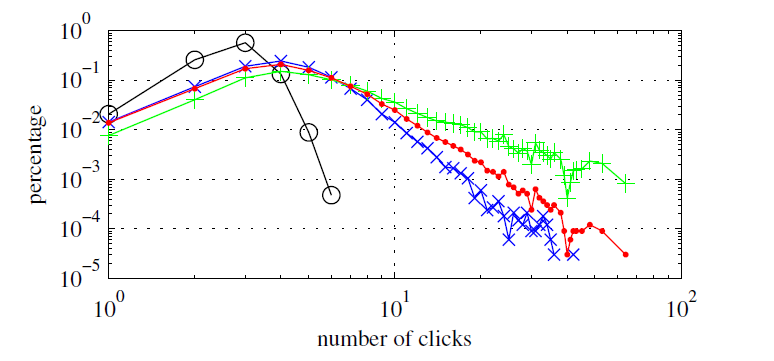
\includegraphics{number of clicks.png}}
\caption{The distribution of Wikispeedia game length, according to different path length metrics }
\label{fig}
\end{figure} \\
We find the length of the shortest path between two articles using shortest-path-distance-matrix.txt. We then find the ratio of the human path and the shortest path for each path mentioned in paths-finished.tsv. We do this process once considering all the back clicks, and then once ignoring all the back clicks. The analysis reveals this information:
\begin{itemize}
\item Humans seldom followed the shortest path.
\item Humans made mistakes during navigation and some regretted it later and backtracked.
\item If we ignore the back clicks made by humans, it is equivalent to paths having no human mistakes, and hence the ratio of the lengths of the human paths and the shortest paths improves.
\end{itemize}
\subsection{Question 7.}
On analyzing the results of this question, we can see that a major percentage of human paths are longer than the shortest path, with only 22.37\% of them having the same length as the shortest path.  It can also be seen that the human path lengths, on average are 6.28 compared to 3.88 for the shortest path lengths. \\

Using the histograms shown in figure 2 and figure 3, we can see that most of the human paths are less than 10 links long, but they can range up to 30 links long. In contrast, the shortest path lengths are only between 1 to 7 links long.\\
\begin{figure}[htbp]
\centerline{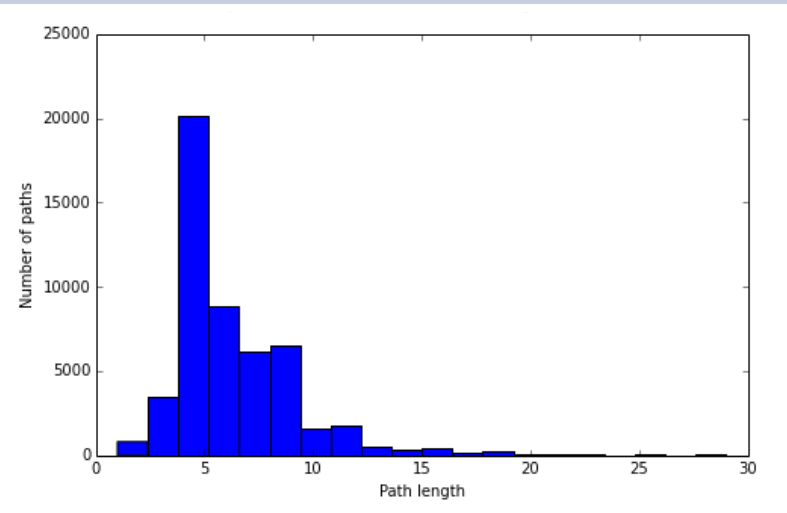
\includegraphics{human paths.png}}
\caption{Histogram of human path lengths with average: 6.28}
\label{fig}
\end{figure} \\
\begin{figure}[htbp]
\centerline{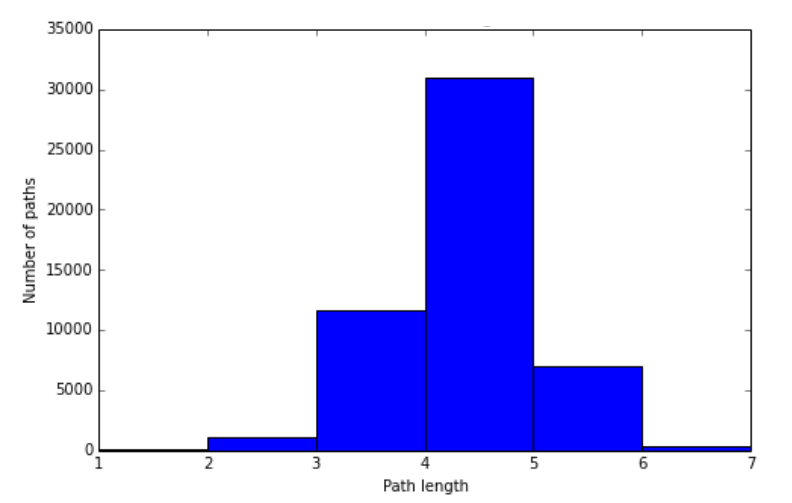
\includegraphics{shortest paths.png}}
\caption{Histogram of shortest path lengths with average: 3.88}
\label{fig}
\end{figure} \\
\newpage
\subsection{Question 8.}
The analysis here reveals how often is a category visited in each human path as well as its corresponding shortest path. We can observe that the category \textit{subject.Countries} is visited most number of times.
\subsection{Question 9.}
Here, we extend the above analysis to include even the subcategories of articles. We can see that the subcategory \textit{subject.Geography} is the second most visited category after the subcategory \textit{subject} which is the root of the category tree.
\subsection{Question 10 and 11.}
We compute the source destination category pairs, first for unfinished paths, and then for finished paths. We find the percentage of finished and unfinished paths for each category pair and  we then find the average ratio of length of human (without back clicks) paths to shortest paths. It can be seen that the category pair \textit{subject.Everyday\_life.Films, subject.Language\_and\_literature.Literature\_types} have the longest human to shortest path ratio of 17.66.
\section{Conclusions}
Using the analysis done so far, we can draw the following conclusions:
\begin{enumerate}
\item Humans manage to find ‘short' paths. Players naturally have no knowledge of Wikipedia’s structure, yet they achieve short search times through locally greedy behavior,
leveraging their background knowledge to determine which outgoing links of the
current article are most promising to decrease the distance to the target. 
\item Human paths rarely follow the ‘shortest' path length.
\item The Wikipedia graph is an example of a ‘small world’ in which most pairs of nodes are
connected by short chains, with an average shortest-path length  across all pairs of 3.28. Wikipedia’s hyperlink graph is structured in a way that is conducive to
making local, greedy navigation strategies successful, through its nearly perfect mix of short- and long-range semantic connections.
\item Humans often make mistakes, and regret them later, as revealed by the back clicks in human paths.
\item Humans tend to give up, often because they fail to reach the destination node in a reasonable amount of time, and often due to other factors as well.
\end{enumerate}
\end{document}
